% How the strategist (the archivist) decides: its rules pick a role, the engage role is a
% short look-ahead search, and the rules are read again whenever a move ends.
% Data: data/pilots.json "archivist"; Tree and Search in crates/pilot/src/lib.rs.
% Standalone: compiles on its own in Overleaf with pdflatex.
\documentclass[tikz,border=4pt]{standalone}
\usetikzlibrary{arrows.meta,shapes.geometric,positioning,calc}

% --- Colors: the deck's palette --------------------------------------------
\definecolor{paper}{HTML}{FDFDFC}   % node fill
\definecolor{ink}{HTML}{1B2430}     % text and edges
\definecolor{muted}{HTML}{6B7680}   % notes
\definecolor{cond}{HTML}{2F4BA0}    % conditions and the world it reads
\definecolor{act}{HTML}{2A6B4A}     % moves
\definecolor{intr}{HTML}{8B2E2E}    % interrupts

% --- Settings: the archivist's entry, and the search a tree's engage role runs ----
\newcommand{\Reaction}{6}      % reaction_ticks
\newcommand{\ReactionMs}{100}  % the same in ms
\newcommand{\Horizon}{18}      % ticks each candidate is simulated (Tree::play's Search::new)
\newcommand{\Branches}{11}     % key combinations tried
\newcommand{\Hold}{3}          % ticks it presses the best before searching again
\newcommand{\EngageTicks}{12}  % length of one engage move

% --- Layout, in centimetres --------------------------------------------------
\newcommand{\RuleGap}{4.7}     % distance between the rule boxes
\newcommand{\BarY}{-5.0}       % the bar the rules return along when a move ends
\newcommand{\RuleW}{3.4cm}     % width of a rule box
\newcommand{\RuleY}{-2.6}      % height of the rule boxes
\newcommand{\PipeX}{22.4}      % the search pipeline's column
\newcommand{\PipeGap}{1.55}    % vertical distance between pipeline steps

\begin{document}
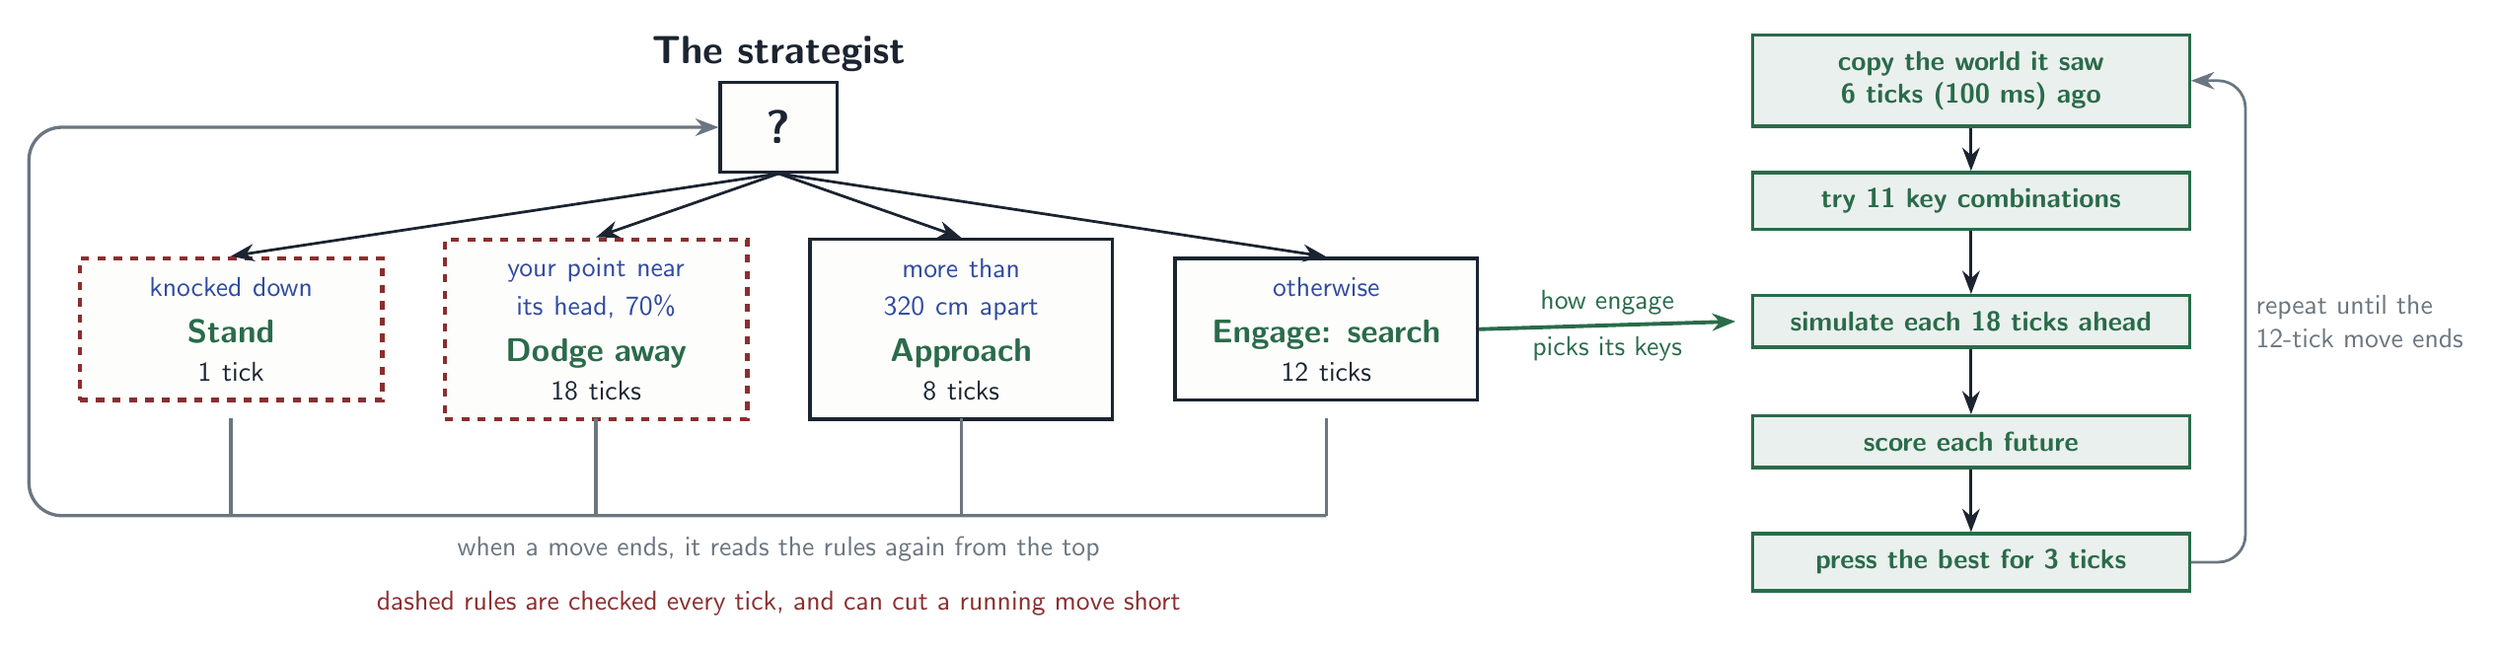
\begin{tikzpicture}[
    font=\sffamily\large, ink,
    edge/.style={-{Stealth[length=3mm]}, line width=1pt, draw=ink},
    selector/.style={draw=ink, line width=1.2pt, fill=paper, minimum width=1.5cm, minimum height=1.15cm, font=\sffamily\bfseries\LARGE},
    rule/.style={draw=ink, line width=1.2pt, fill=paper, text width=\RuleW, align=center, inner sep=7pt},
    intrrule/.style={rule, draw=intr, dashed, line width=1.6pt},
    pipestep/.style={draw=act, line width=1.2pt, fill=act!10, text=act, text width=5.2cm, align=center, inner sep=6pt, font=\sffamily\normalsize\bfseries},
  ]

% --- The strategy layer: rules in priority order ------------------------------------
\node[selector] (root) at (1.5*\RuleGap, 0) {?};
\node[anchor=south, font=\sffamily\bfseries\Large] at (root.north) {The strategist};
\foreach \i/\cond/\move/\ticks/\style in {
    0/{knocked down}/{Stand}/{1 tick}/intrrule,
    1/{your point near its head, 70\%}/{Dodge away}/{18 ticks}/intrrule,
    2/{more than 320 cm apart}/{Approach}/{8 ticks}/rule,
    3/{otherwise}/{Engage: search}/{\EngageTicks{} ticks}/rule} {
  \node[\style] (r\i) at (\i*\RuleGap, \RuleY) {{\color{cond}\normalsize\cond}\\[3pt]{\color{act}\bfseries\move}\\{\normalsize\ticks}};
  \draw[edge] (root.south) -- (r\i.north);
}

% --- Reassignment: the rules are read again when a move ends ---------------------------
\foreach \i in {0,...,3} {
  \draw[muted, line width=1.2pt] (r\i.south |- 0,\RuleY-1.15) -- (\i*\RuleGap, \BarY);
}
\draw[edge, muted, line width=1.2pt, rounded corners=12pt]
  (3*\RuleGap, \BarY) -- (-2.6, \BarY) |- (root.west);
\node[anchor=north, text=muted, font=\sffamily\normalsize] at (1.5*\RuleGap, \BarY-0.15)
  {when a move ends, it reads the rules again from the top};
\node[anchor=north, text=intr, font=\sffamily\normalsize] at (1.5*\RuleGap, \BarY-0.85)
  {dashed rules are checked every tick, and can cut a running move short};

% --- Unit control for engage: the search, opened up -------------------------------------
\foreach \k/\text in {0/{copy the world it saw \Reaction{} ticks (\ReactionMs{} ms) ago},
                      1/{try \Branches{} key combinations},
                      2/{simulate each \Horizon{} ticks ahead},
                      3/{score each future},
                      4/{press the best for \Hold{} ticks}} {
  \node[pipestep] (p\k) at (\PipeX, 0.6 - \k*\PipeGap) {\text};
}
\foreach \k [evaluate=\k as \n using int(\k+1)] in {0,...,3} {
  \draw[edge] (p\k.south) -- (p\n.north);
}
\draw[edge, act, line width=1.4pt] (r3.east) -- node[above, font=\sffamily\normalsize, text=act] {how engage} node[below, font=\sffamily\normalsize, text=act] {picks its keys} ($(p2.west)+(-0.2,0)$);
\draw[edge, muted, rounded corners=10pt] (p4.east) -- ++(0.7,0) |- node[pos=0.25, right, text=muted, font=\sffamily\normalsize, align=left] {repeat until the\\\EngageTicks-tick move ends} (p0.east);

\end{tikzpicture}
\end{document}

% --- Self-check ----------------------------------------------------------------
% Rules: the \foreach list is data/pilots.json's "archivist" rules in order; the two with
%   "interrupt": true are dashed (intrrule).
% Lengths: stand 1, dodge_away 18, approach 8, search 12 ticks: Tree::play.
% Search: Tree::play builds Search::new(18, reaction, 11, 3): \Horizon, \Reaction, \Branches,
%   \Hold; it decides on the world \Reaction ticks old.
% Lengths are written out ("1 tick", "N ticks"). The rule boxes' bottoms drop to the bar at
%   \BarY, which returns to the root's side: the reassignment.
% Reassignment: Tree::input picks a new move when the current one returns None, and checks
%   interrupt rules every tick while a move runs.
